% ---- this is the preamble
\documentclass[a4paper]{scrartcl}

\usepackage[french,english]{babel}%langue française
\usepackage[utf8]{inputenc} %utilisation des accents
\usepackage{amsmath,amssymb,amsfonts,lscape}
%\usepackage{siunitx}
\usepackage{graphicx}
\usepackage{tabularx}
\usepackage[square, comma, sort&compress]{natbib}

\usepackage{microtype} % Slightly tweak font spacing for aesthetics

\usepackage[hmarginratio=1:1,top=3cm, right=3cm,columnsep=6mm]{geometry} % Document margins
\usepackage[hang, small,labelfont=bf,up,textfont=it,up]{caption} % Custom captions under/above floats in tables or figures
\usepackage{booktabs} % Horizontal rules in tables
\usepackage[colorlinks=true, citecolor=red]{hyperref} % For hyperlinks in the PDF
\usepackage{cleveref}

\usepackage{paralist} % Used for the compactitem environment which makes bullet points with less space between them

\usepackage{listings} %include the source code.
%frame=single, keepspaces=true, basicstyle=\normalsize\ttfamily

\lstset{ %
	frame=single,
	basicstyle=\normalsize\ttfamily,
	escapeinside={\%*}{*)}
}

\usepackage{abstract} % Allows abstract customization
%\renewcommand{\abstractnamefont}{\normalfont\bfseries} % Set the "Abstract" text to bold
\renewcommand{\abstracttextfont}{\normalfont\normalsize} % Set the abstract itself to small italic text
\addto\captionsenglish{\renewcommand*\abstractname{Summary}}


\def\mytitle{\@title}

%Define headers and footers.
\usepackage{fancyhdr} % Headers and footers
\pagestyle{fancy} % All pages have headers and footers
\fancyhead{} % Blank out the default header
\fancyfoot{} % Blank out the default footer
\fancyhead[C]{\textsf{Documentation ECCW}} %\includegraphics[height=2.5mm]{../Pictures/id2_slamtec_mate.pdf} }
%\fancyhead[R]{\today}
\fancyfoot[C]{\thepage} % Custom footer text
\headsep=1.5cm
%Redefine maketitle
\makeatletter
\def\@maketitle{%
	\begin{center}%
		\large{\textbf{\textsf{DOCUMENTATION}}}\\ 		
		\hrulefill\\
		\vspace{2mm}
		
\includegraphics[width=12cm]{eccw_title.png}\\
%		
\includegraphics[width=3cm]{icon_eccw.pdf}\\
		\vspace{2mm}    
		{\Huge \textsf\@subtitle}\\
		\vspace{5mm}%
		{\large\@author}\\%
		\vspace{5mm}%
		{\Large \@date}%
	\end{center}%
	\par
	\vspace{5mm}
}
\makeatother


%\newcommand{\pathfig}{/home/bmary/Figures}
\graphicspath{{images/}}

%-----------------------------------------------------------------------------

\newcommand{\mat}[1]{\underline{\underline{#1}}}
\renewcommand{\vec}[1]{\underline{#1}}

%----------------------------------------------------------------------------------------


\title{ECCW} 
\subtitle{Exact Critical Coulomb Wedge}


\author{B.C.L. Mary}

%------------------------------- beginning of the document
\begin{document}


\maketitle % Insert title

\begin{abstract}

ECCW is a python library and a GUI of this library.
The ECCW python library allows to compute the exact solution of critical Coulomb wedge, draw it, sketch it, with love.
Are available compressive or extensive geological context, with or without fluid pore pressure.

\end{abstract}

\setcounter{tocdepth}{2}
\tableofcontents

%-----------------------------------------------------------------------------------------------------------
\newpage
\section{Usage}
%-----------------------------------------------------------------------------------------------------------

\begin{lstlisting} 
main.py [-h] [-V] [-d] [-f FILE]
\end{lstlisting}

%The ECCW application gets a maximum of 6 positional parameters. 
%According to the number of given parameters, the result is different.
%Two main behaviours are to expect :
%\begin{itemize}
%	\item compute the critical surface slope $\alpha_c$,
%	\item draw the complete enveloppe of the critical domain.
%\end{itemize}
%Additionnaly, four optionals arguments can be used :
%\begin{description}
%	\item[\texttt{--file}] : ploting a list of specific nodes ;
%	\item[\texttt{--nodraw}] : disable ploting (for command line workflow purpose) ;
%	\item[\texttt{--box}] : set limits of plot ; 
%	\item[\texttt{--sketch}] : draw sketches of the wedge with faults orientations and directions.
%\end{description}
%
%%-----------------------------------------------------------------------------------------------------------
%\subsection{Compute critical surface slope $\alpha_c$}
%
%To obtain the \emph{value} of the critical slope for a given set of parameters, just mind to give the angle of the décollement \texttt{beta} at the end of the given parameters.
%\\
%
%\subsubsection{Dry case}
%
%For dry case, three parameters are expected in following order :
%\begin{description}
%	\item[\texttt{phi\_B}] : bulk friction angle $\phi_B$ in degree ;
%    \item[\texttt{phi\_D}] : friction angle of décollement $\phi_D$ in degree ;
%    \item[\texttt{beta}] : slope of décollement $\beta$ in degree.
%\end{description}
%\begin{lstlisting}[title=example]
%$ eccw 30 10 3
%alphac = 1.4403 or 26.3795
%\end{lstlisting}
%With the solution, a window pop out with a plot of the complete solution (Figure \ref{fig:example_dry}).
%A vertical line illustrate the value of asked basal slope $\beta$, with two black dots at its intersection with the critical enveloppe.
%See section \ref{sec:understand_ECCW} for physical meaning of results. 
%
%\begin{figure}[h]
%	\centering
%	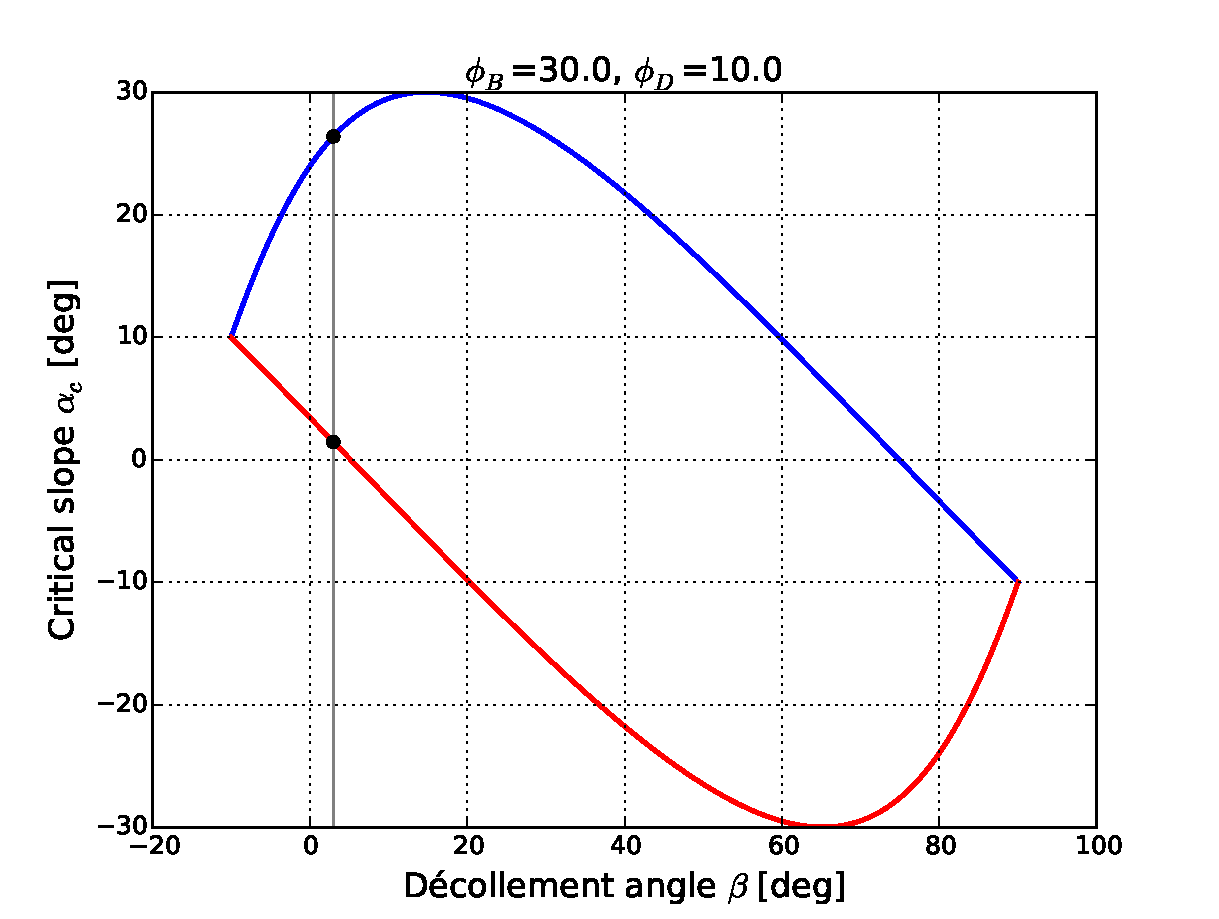
\includegraphics[width=10cm]{ECCW_example_dry.pdf}
%	\caption{Example of plot obtained with the computation of the critical surface, for dry case.}
%	\label{fig:example_dry}
%\end{figure}
%
%If the asked value of \texttt{beta} has no possible solution for the given parameters, a simple message tells it.
%The plot of the critical enveloppe helps to diagnose such a response using the position of the vertical black line (try to set \texttt{beta} to -15 in previous example).
%\\
%
%For some reasons, the user may want to obtain the solution alone, without any plot.
%In that case the argument \texttt{--nodraw} can be added.
%\begin{lstlisting}[title=example]
%$ eccw 30 10 3 --nodraw
%\end{lstlisting}
%
%\subsubsection{With fluids}
%For fluid pore pressure case (see Figure \ref{fig:example_fluids}), six parameters are expected in following order :
%\begin{description}
%	\item[\texttt{phi\_B}] : bulk friction angle $\phi_B$ (in degree) ;
%    \item[\texttt{phi\_D}] : friction angle of décollement ($\phi_D$ in degree) ;
%    \item[\texttt{delta\_lambda\_B}] : bulk fluid overpressure gradient $\Delta \lambda_B \in [0 : 1 - \frac{\rho_f}{\rho} [$. This is the deviation from pure hydrostatic pore pressure profile ;
%    \item[\texttt{delta\_lambda\_D}] : décollement fluid overpressure gradient $\Delta \lambda_D \in [0 : 1 - \frac{\rho_f}{\rho} ]$ ;
%    \item[\texttt{density\_ratio}] : ratio of fluid density $\rho_f$ ($\sim1000$) and saturated rock density $\rho \in [1100 : 3000]$ ;
%    \item[\texttt{beta}] : slope of décollement $\beta$ in degree.
%\end{description}
%\begin{lstlisting}[title=example]
%$ eccw 30 10 0.5 0.4 0.42 3
%alphac = 1.9711 or 3.4732
%\end{lstlisting}
%\begin{figure}[h]
%	\centering
%	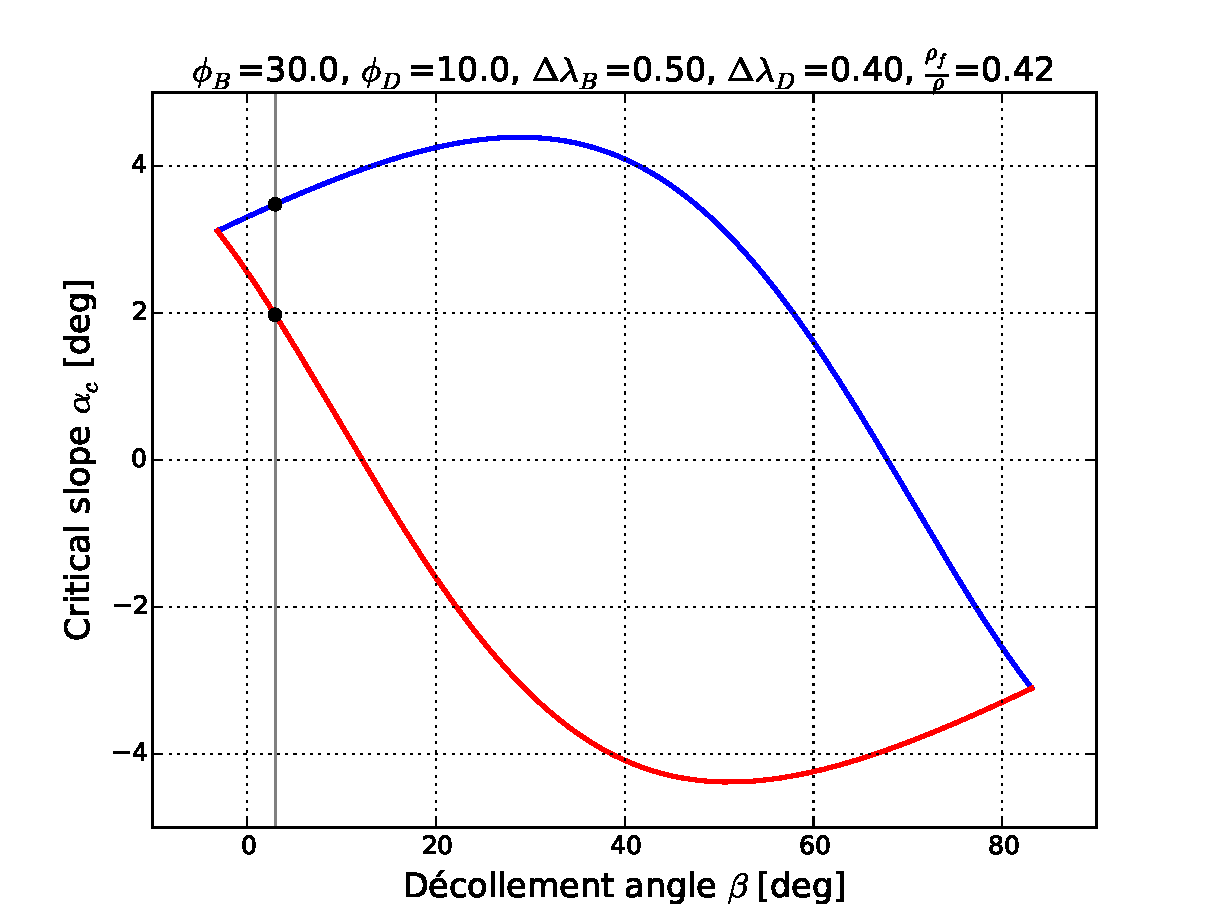
\includegraphics[width=10cm]{ECCW_example_fluids.pdf}
%	\caption{Example of plot obtained with the computation of the critical surface, for case with fluids.}
%	\label{fig:example_fluids}
%\end{figure}
%
%%-----------------------------------------------------------------------------------------------------------
%\subsection{Tectonic context}
%
%Computation or display of critical surface slope is available for compressive or extensive tectonic context.
%Default context is compressive.
%To obtain a result in extensive context, the user had to set a \emph{negative} value to the parameter \texttt{phi\_D} (friction angle on décollement $\phi_D$).
%
%\begin{lstlisting}[title=example]
%$ eccw 30 -10 12 --nodraw
%alphac = -11.2839 or -6.2474
%\end{lstlisting}
%
%%-----------------------------------------------------------------------------------------------------------
%\subsection{Complete enveloppe of the critical domain}
%
%For both cases, dry and with fluids, when last parameter $\beta$ is ommited, only the plot of the critical enveloppes are displayed.
%\begin{lstlisting}[title=example]
%$ eccw 30 10
%
%$ eccw 30 10 0.5 0.4 0.42
%\end{lstlisting}
%
%Three optional display arguments are discribed in what follows. 
%All of them can be used combined alltogether and of course combined with a \texttt{beta} value.
%
%\subsubsection{Plot reference points}
%
%Optional argument \texttt{--ECCWfile} plots a collection of points given in a file in given parameter (see Figure \ref{fig:example_file}).
%The file as to be set with (x, y) coordinates into two columns.
%Optionally, color and diameter of the point can be added in third and fourth columns.
%Colors are given by classic key letter (b for blue, y for yellow, k for black, ...).
%Diameters are given in pixels (default is 50).
%\begin{lstlisting}[title=file example]
% 1    5. 
% 5.   2.3  b
%-0.2  3    y  100
%\end{lstlisting}
%\begin{lstlisting}[title=example]
%$ eccw 30 10 --file file-example
%\end{lstlisting}
%\begin{figure}[h]
%	\centering
%	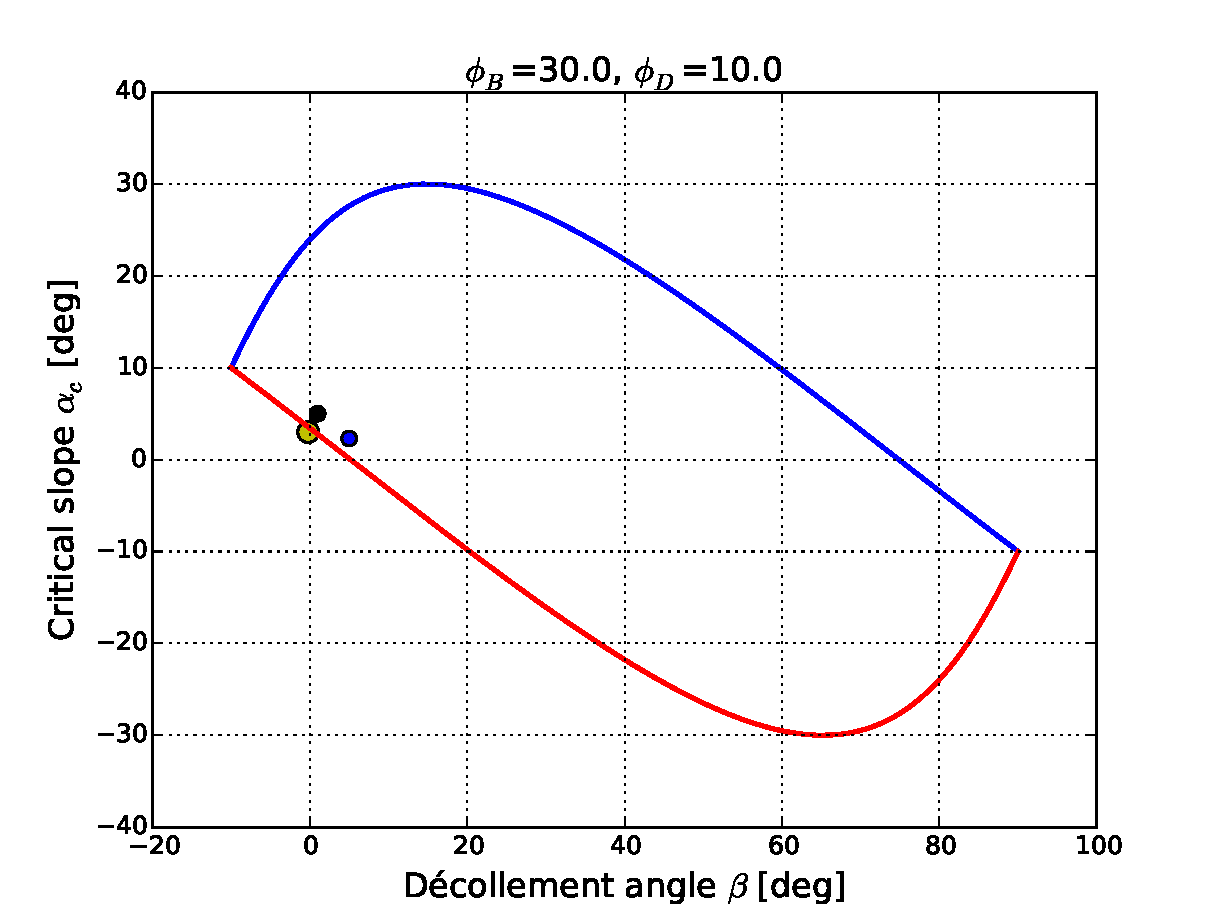
\includegraphics[width=10cm]{ECCW_example_file.pdf}
%	\caption{Example of plot obtained with \texttt{--ECCWfile} argument : some colored reference points are added.}
%	\label{fig:example_file}
%\end{figure}
%
%\subsubsection{Set limits of plot}
%
%Specify the boundaries of what is displayed is simply done using the argument\texttt{--ECCWbox} followed by coordinates of min x, max x, min y, max y. %(see Figure \ref{fig:example_box}).
%\begin{lstlisting}[title=example]
%$ eccw 30 10 --box -15 10 -10 35
%\end{lstlisting}
%%\begin{figure}[h]
%%	\centering
%%	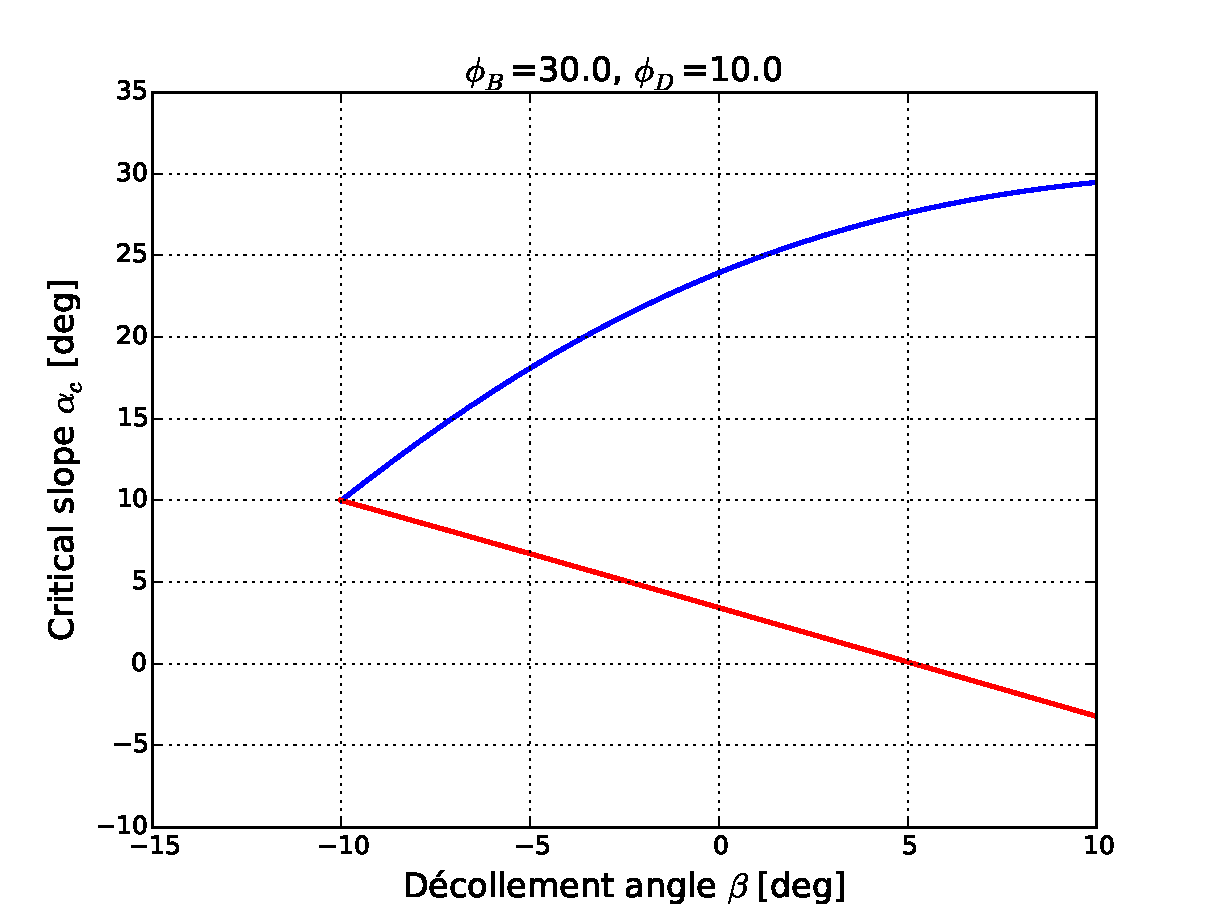
\includegraphics[width=10cm]{ECCW_example_box.pdf}
%%	\caption{Example of plot obtained with \texttt{--ECCWbox} argument : limits of what is diplayed are specified as parameters.}
%%	\label{fig:example_box}
%%\end{figure}
%
%\subsubsection{Drawing sketches of the wedge}
%
%This last option helps a lot to understand the meaning of the given results.
%By simply adding the argument \texttt{--ECCWsection}, real time computed lovely sketches are displayed (see Figure \ref{fig:example_section-comp}).
%These sketches show the orientation of the awaited faults with two set of fine gray lines.
%The direction of these faults is given by the half-arrows.
%The half-arrows on the décollement illustrate the tectonic context (compressive or extensive).
%
%The user may be happy to know that the boxes containing the sketches can be clicked and dropped.
%This help when default positioning is not luckily optimal...
%
%\begin{lstlisting}[title=example]
%$ eccw 30 10 --sketch
%\end{lstlisting}
%
%
%\begin{figure}[p]
%	\centering
%	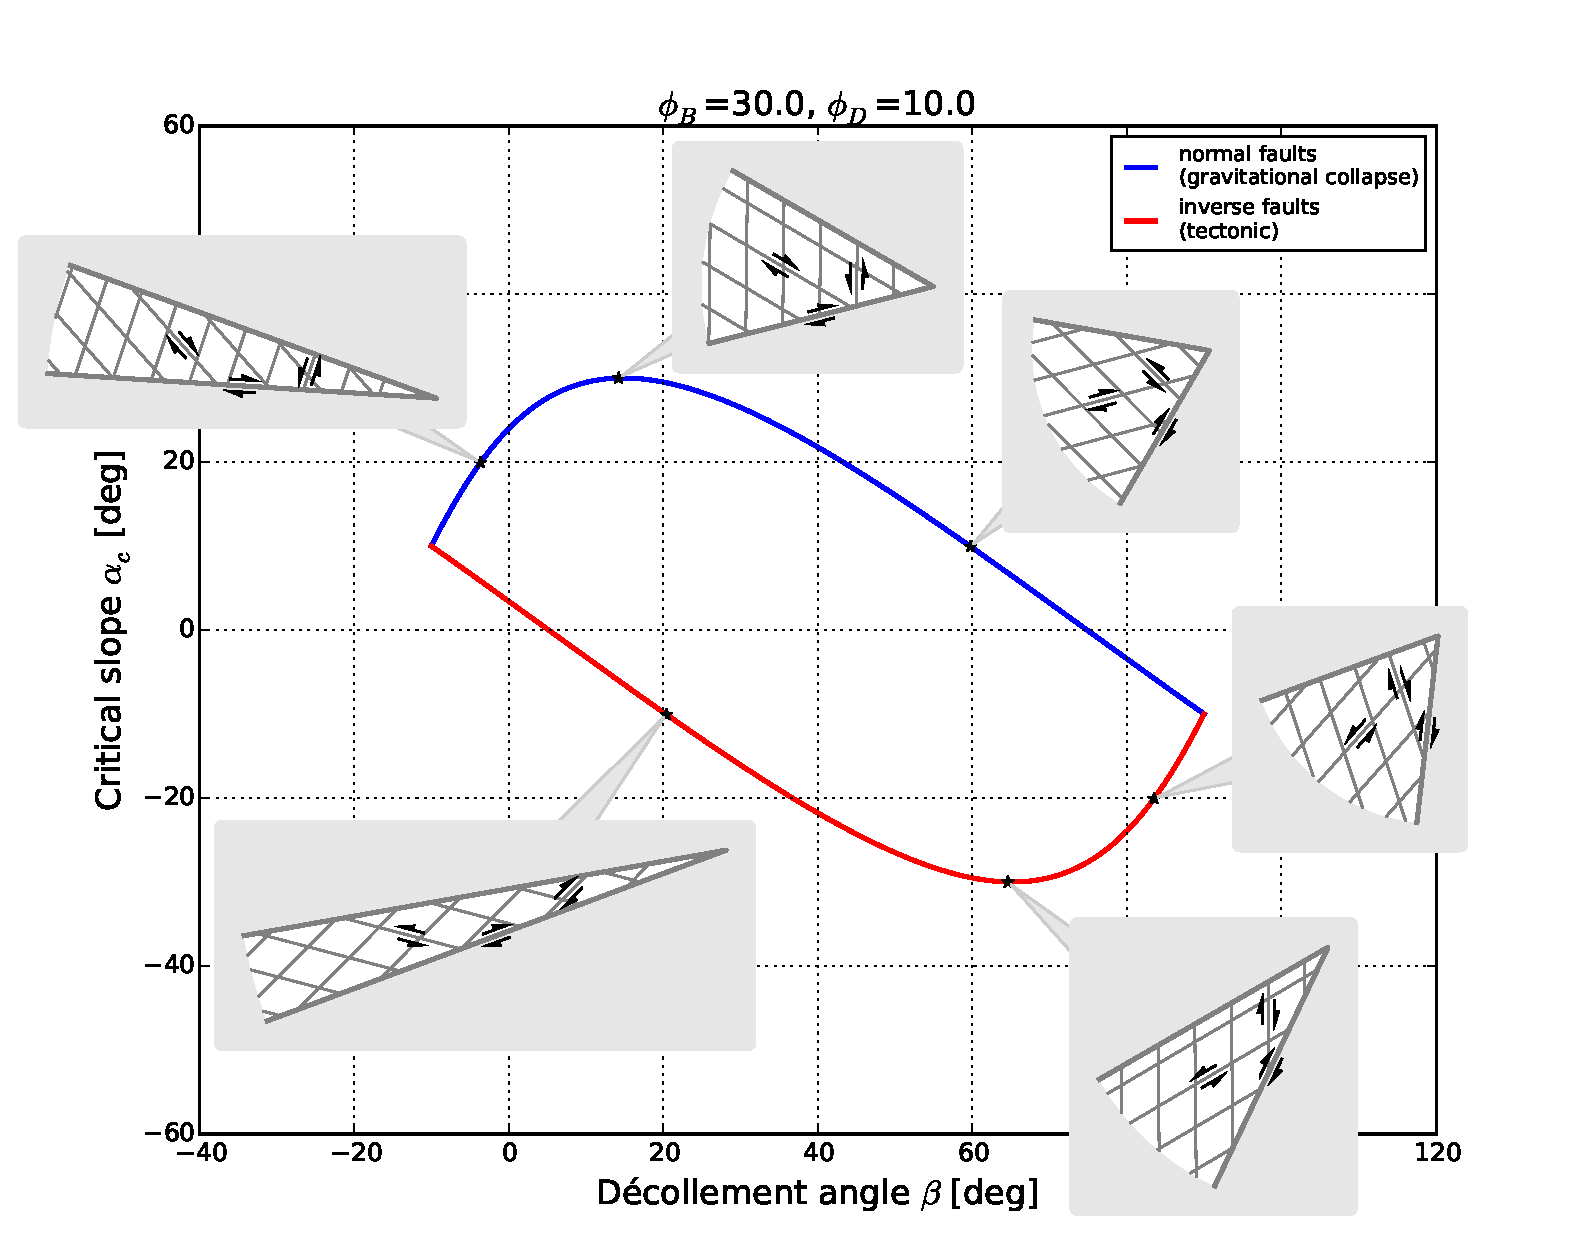
\includegraphics[width=12cm]{ECCW_example_section-comp.pdf}
%	\caption{Example of plot obtained with \texttt{--ECCWsection} argument : sketches of the wedge with the orientation and direction of faults are drawned for caracteristic values.}
%	\label{fig:example_section-comp}
%\end{figure}
%
%\begin{figure}[p]
%	\centering
%	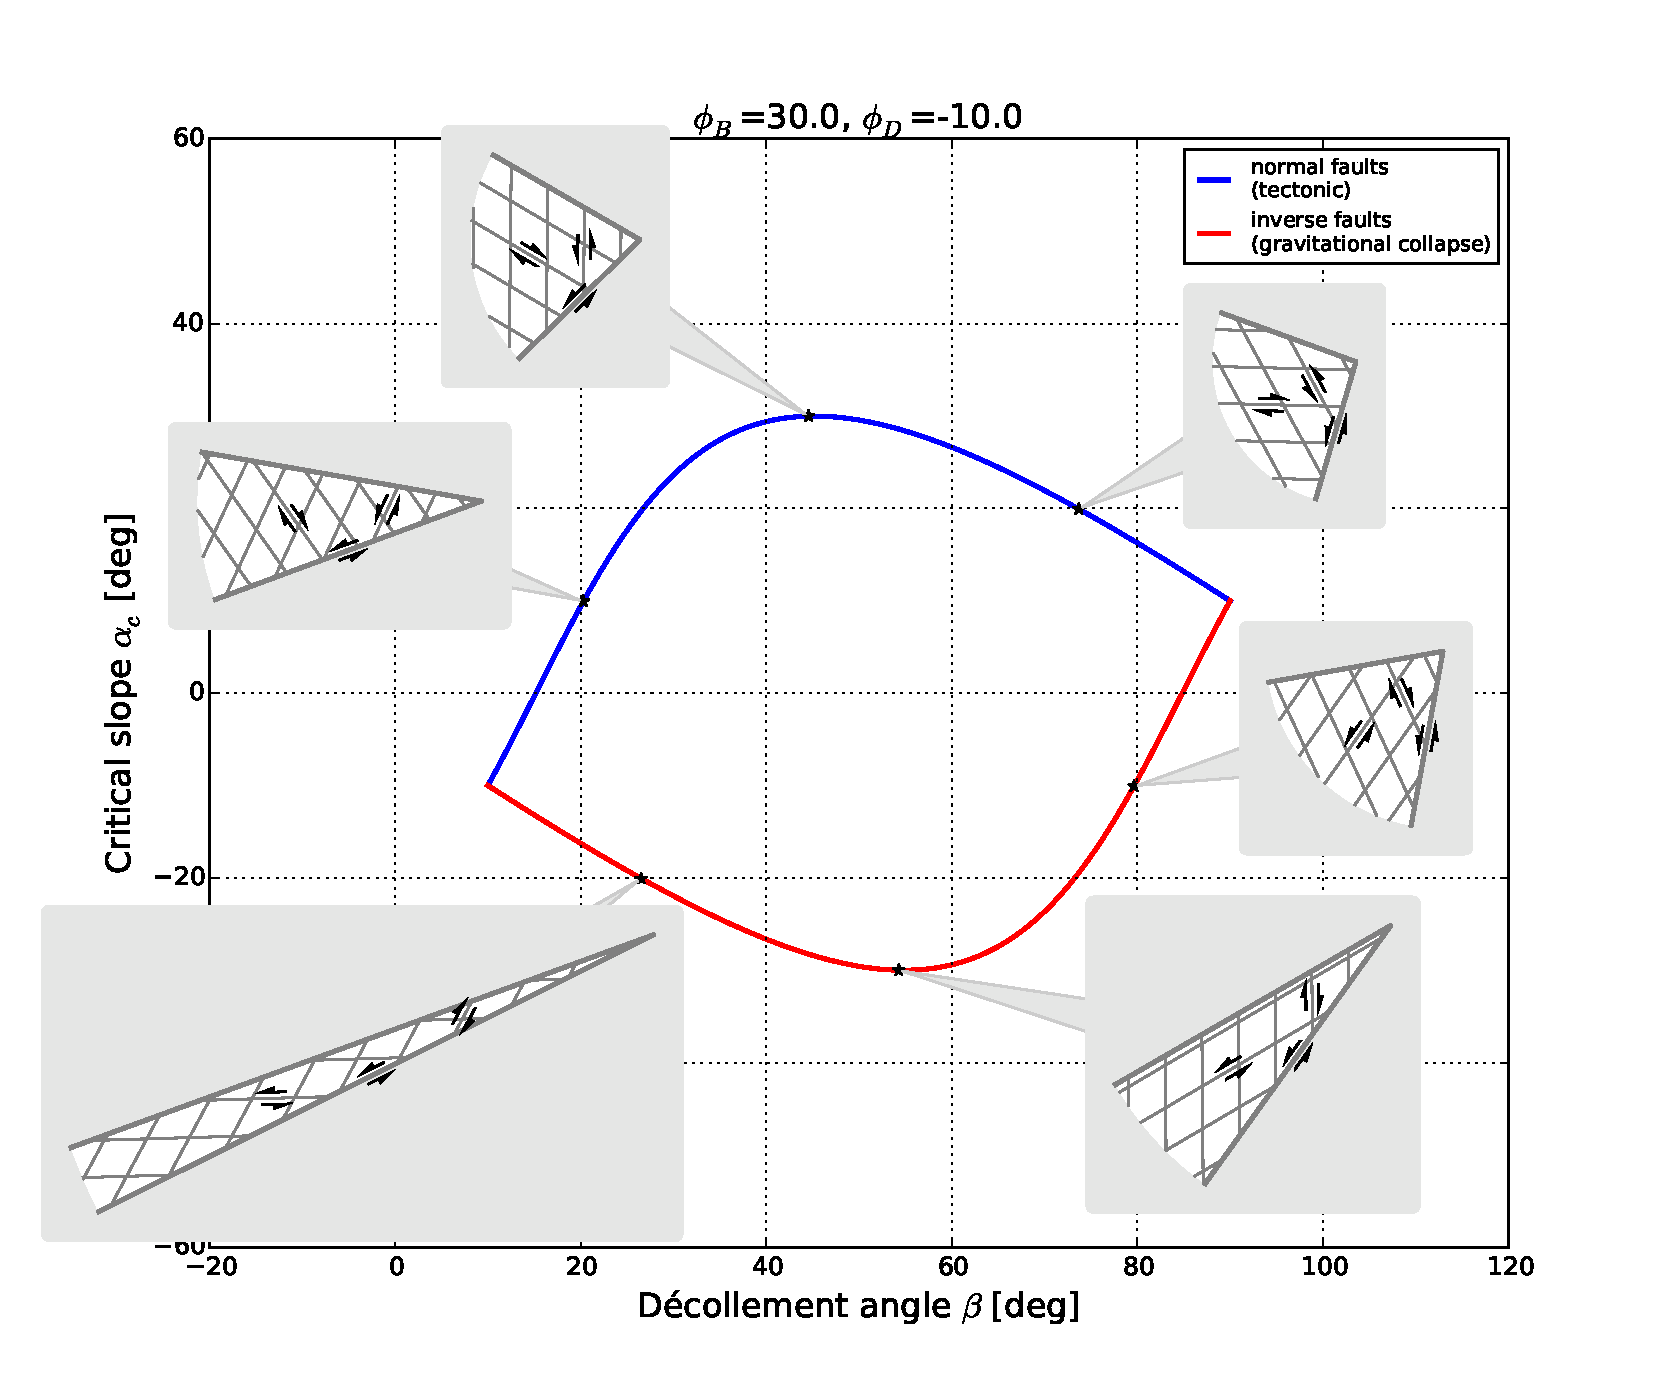
\includegraphics[width=12cm]{ECCW_example_section-ext.pdf}
%	\caption{Example of plot obtained with \texttt{--ECCWsection} in extensive context (negative \texttt{phi\_D} value).}
%	\label{fig:example_section-ext}
%\end{figure}

%-----------------------------------------------------------------------------------------------------------
\newpage
\section{Understand ECCW}
\label{sec:understand_ECCW}
%-----------------------------------------------------------------------------------------------------------

%-----------------------------------------------------------------------------------------------------------
\subsection{The critical coulomb wedge theory.}

\begin{figure}[h]
	\centering
	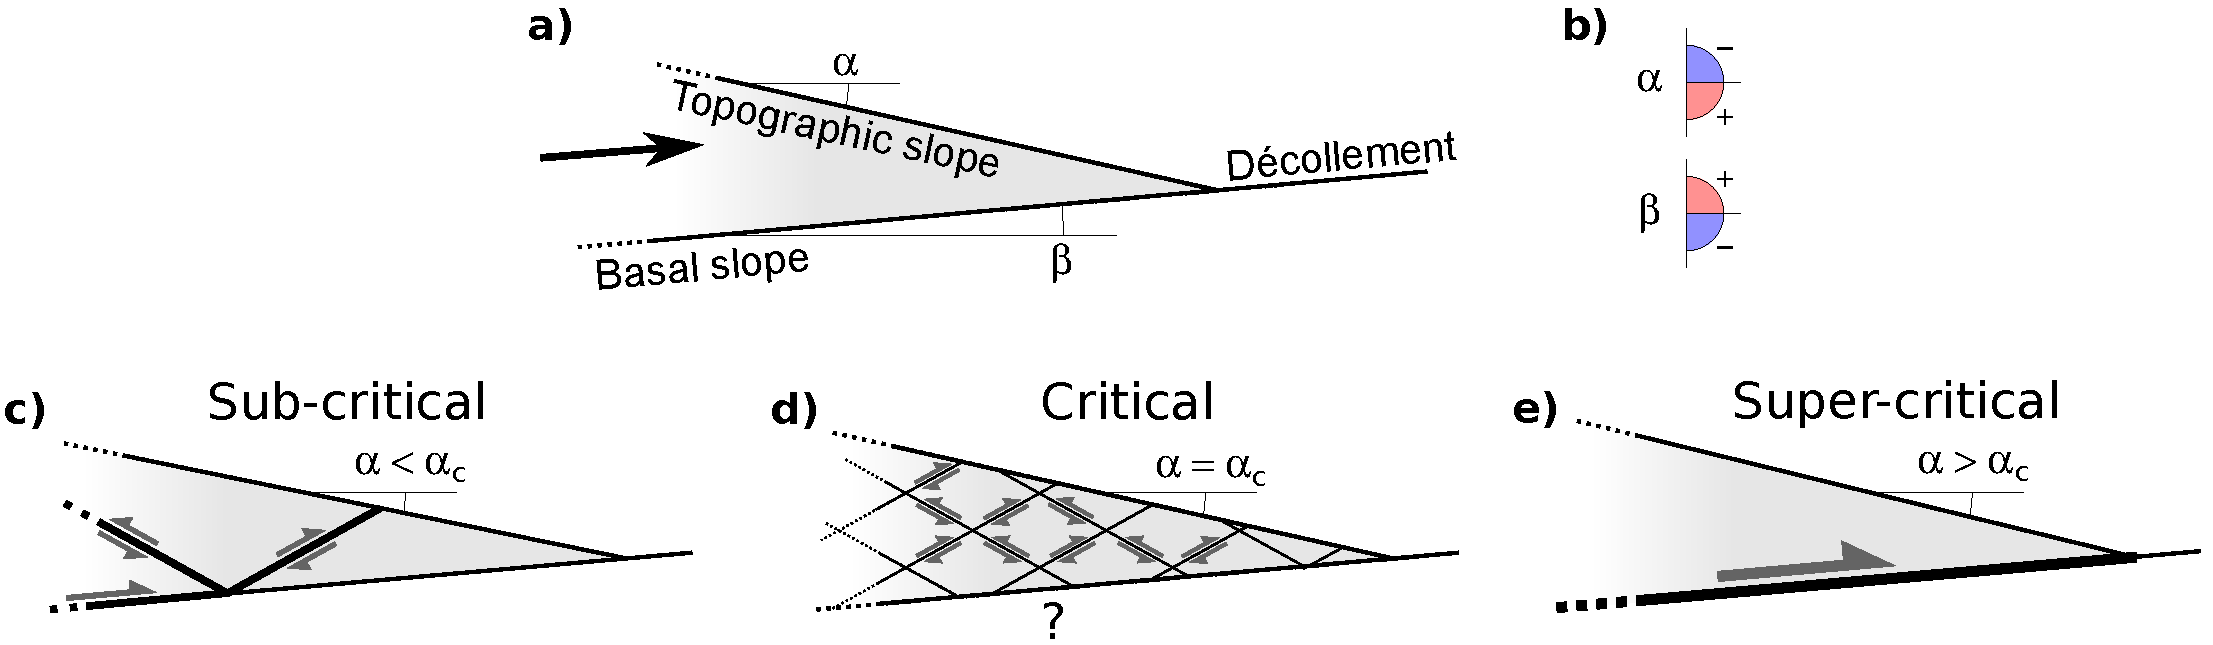
\includegraphics[width=14cm]{Dahlen-geometry.pdf}
	\caption{}
	\label{fig:example_section-ext}
\end{figure}

\begin{figure}[p]
	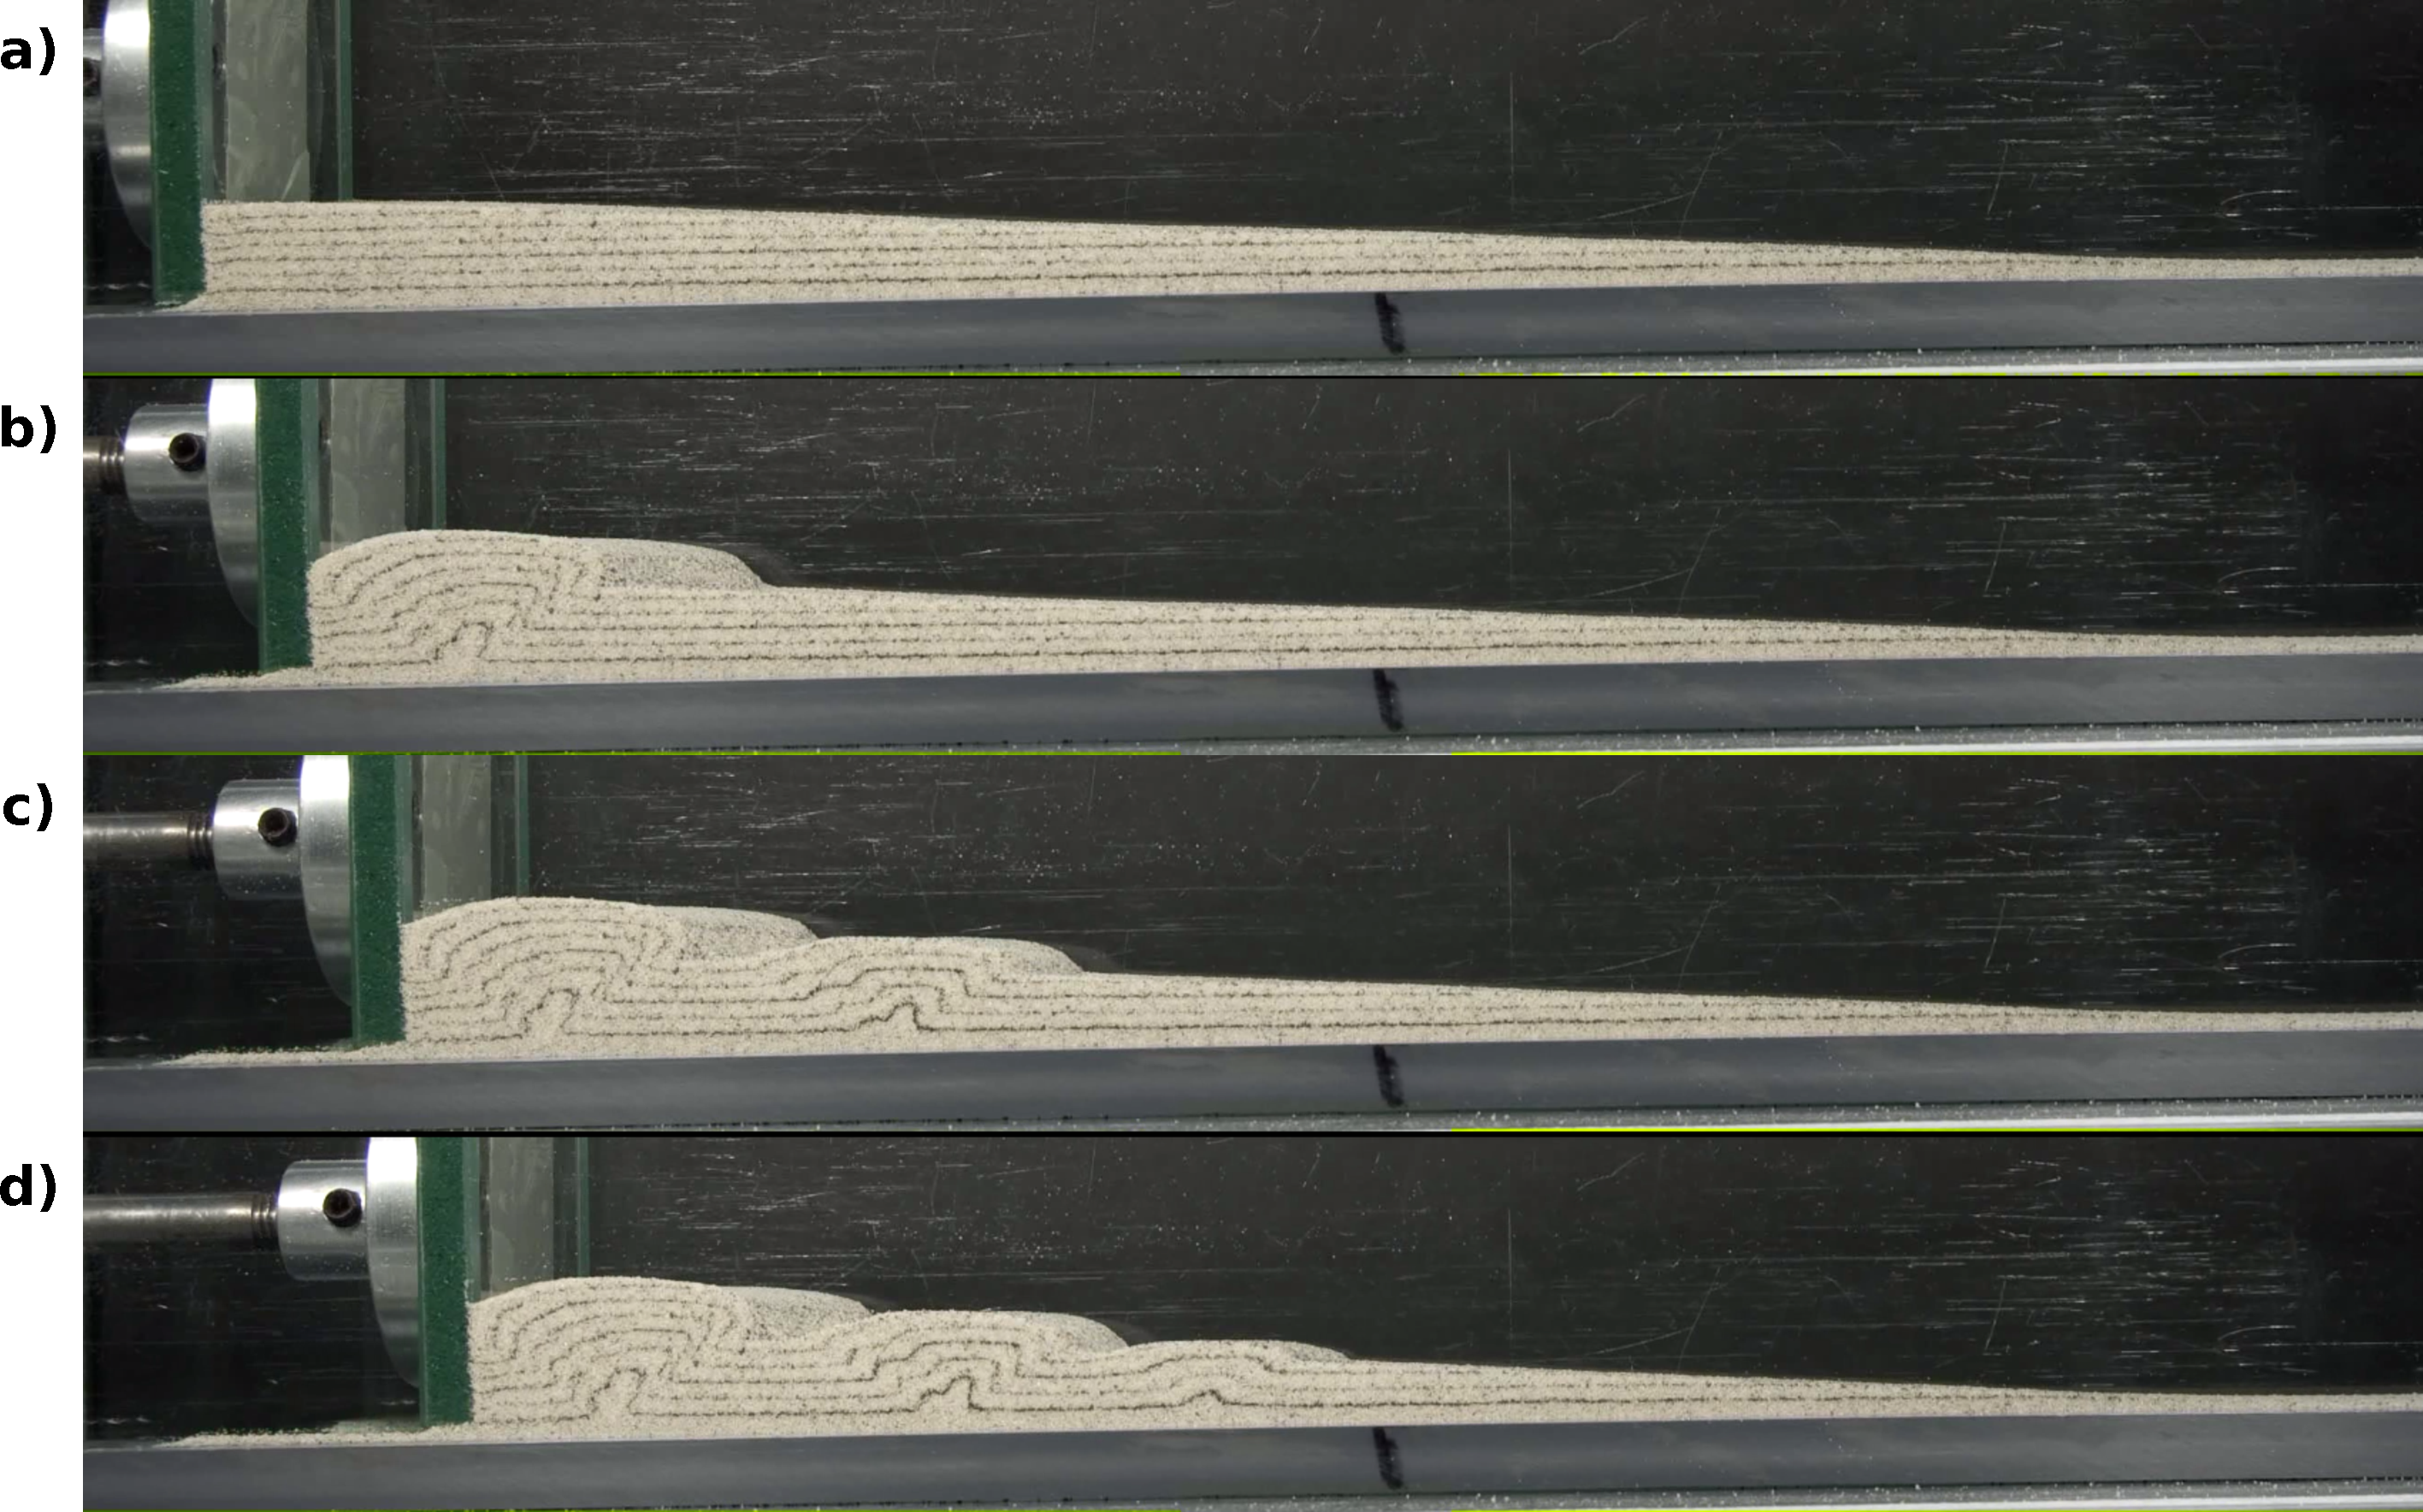
\includegraphics[width=15cm]{Sandbox-subcritical.pdf} 
	\caption{Sandbox experiment showing deformation occuring in a prism initally at sub-critical state (\textbf{a}). Deformation is propagating from the back-wall to the front (\textbf{b} to \textbf{d}). After Souloumiac Thesis, 2009.}
	\label{fig:subcritical}
\end{figure}

\begin{figure}[p]
	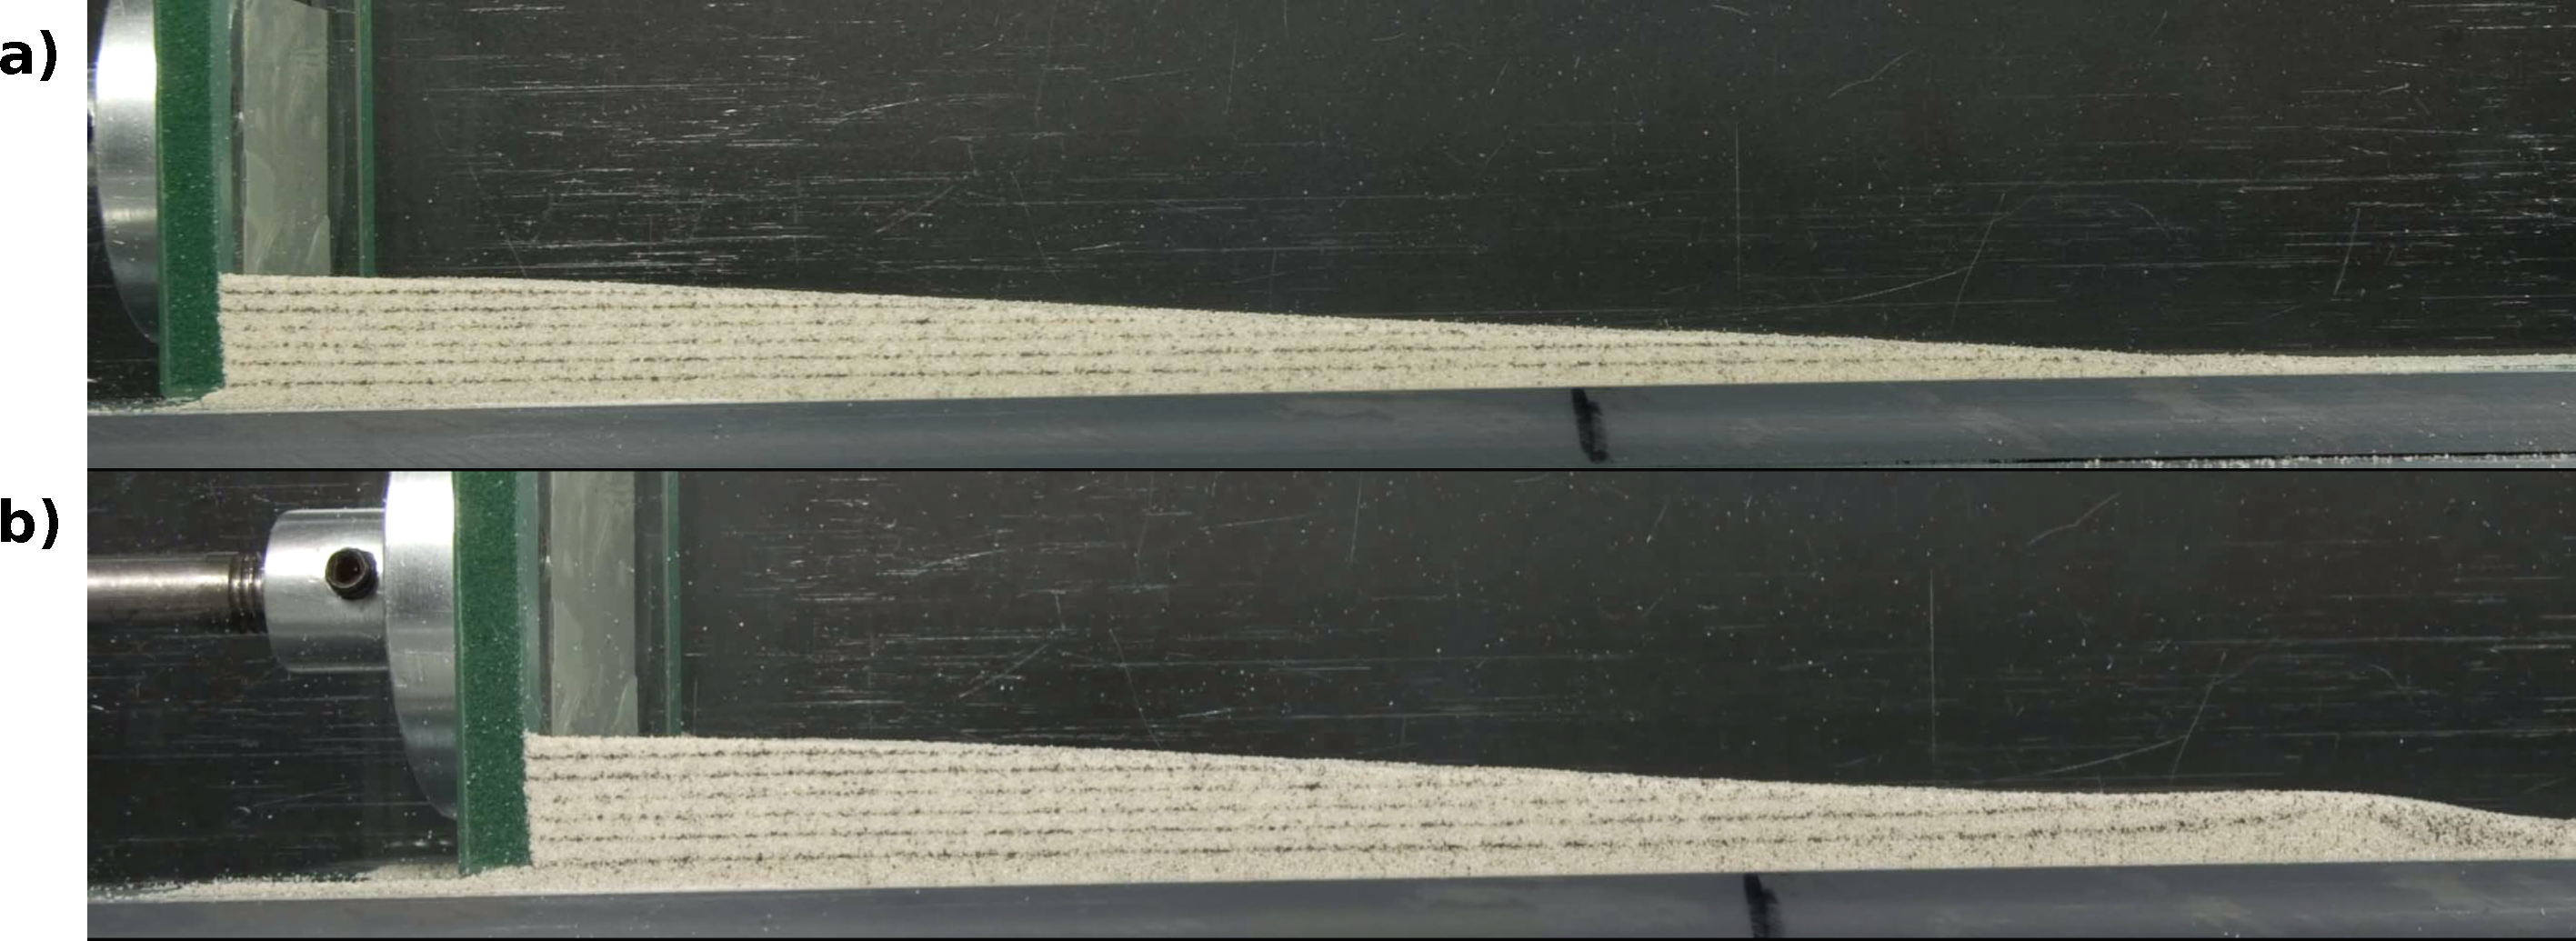
\includegraphics[width=15cm]{Sandbox-supercritical.pdf} 	
	\caption{Sandbox experiment showing no deformation occuring (\textbf{b}) in a prism initally at super-critical state (\textbf{a}). After Souloumiac Thesis, 2009.}
	\label{fig:supercritical}
\end{figure}

%-----------------------------------------------------------------------------------------------------------
\subsection{Criticality.}

The critical enveloppe defines three domains of stability (see figure \ref{fig:domains}):
\begin{itemize}
	\item Super-critical
	\item Sub-critical
	\item Critical
\end{itemize}
In the super-critial doamin, outside the enveloppes, no internal deformation occurs.
The prism only slides on the basal décollement (figure \ref{fig:supercritical}).
In the sub-critical domain, including the enveloppes, some internal deformations occurs.
This deformation will appears along the pushing back-wall in the sub-critical domain (figure \ref{fig:subcritical}), while it can occurs \emph{anywhere} inside the prism at the exact critical state.

\begin{figure}[h]
	\centering
	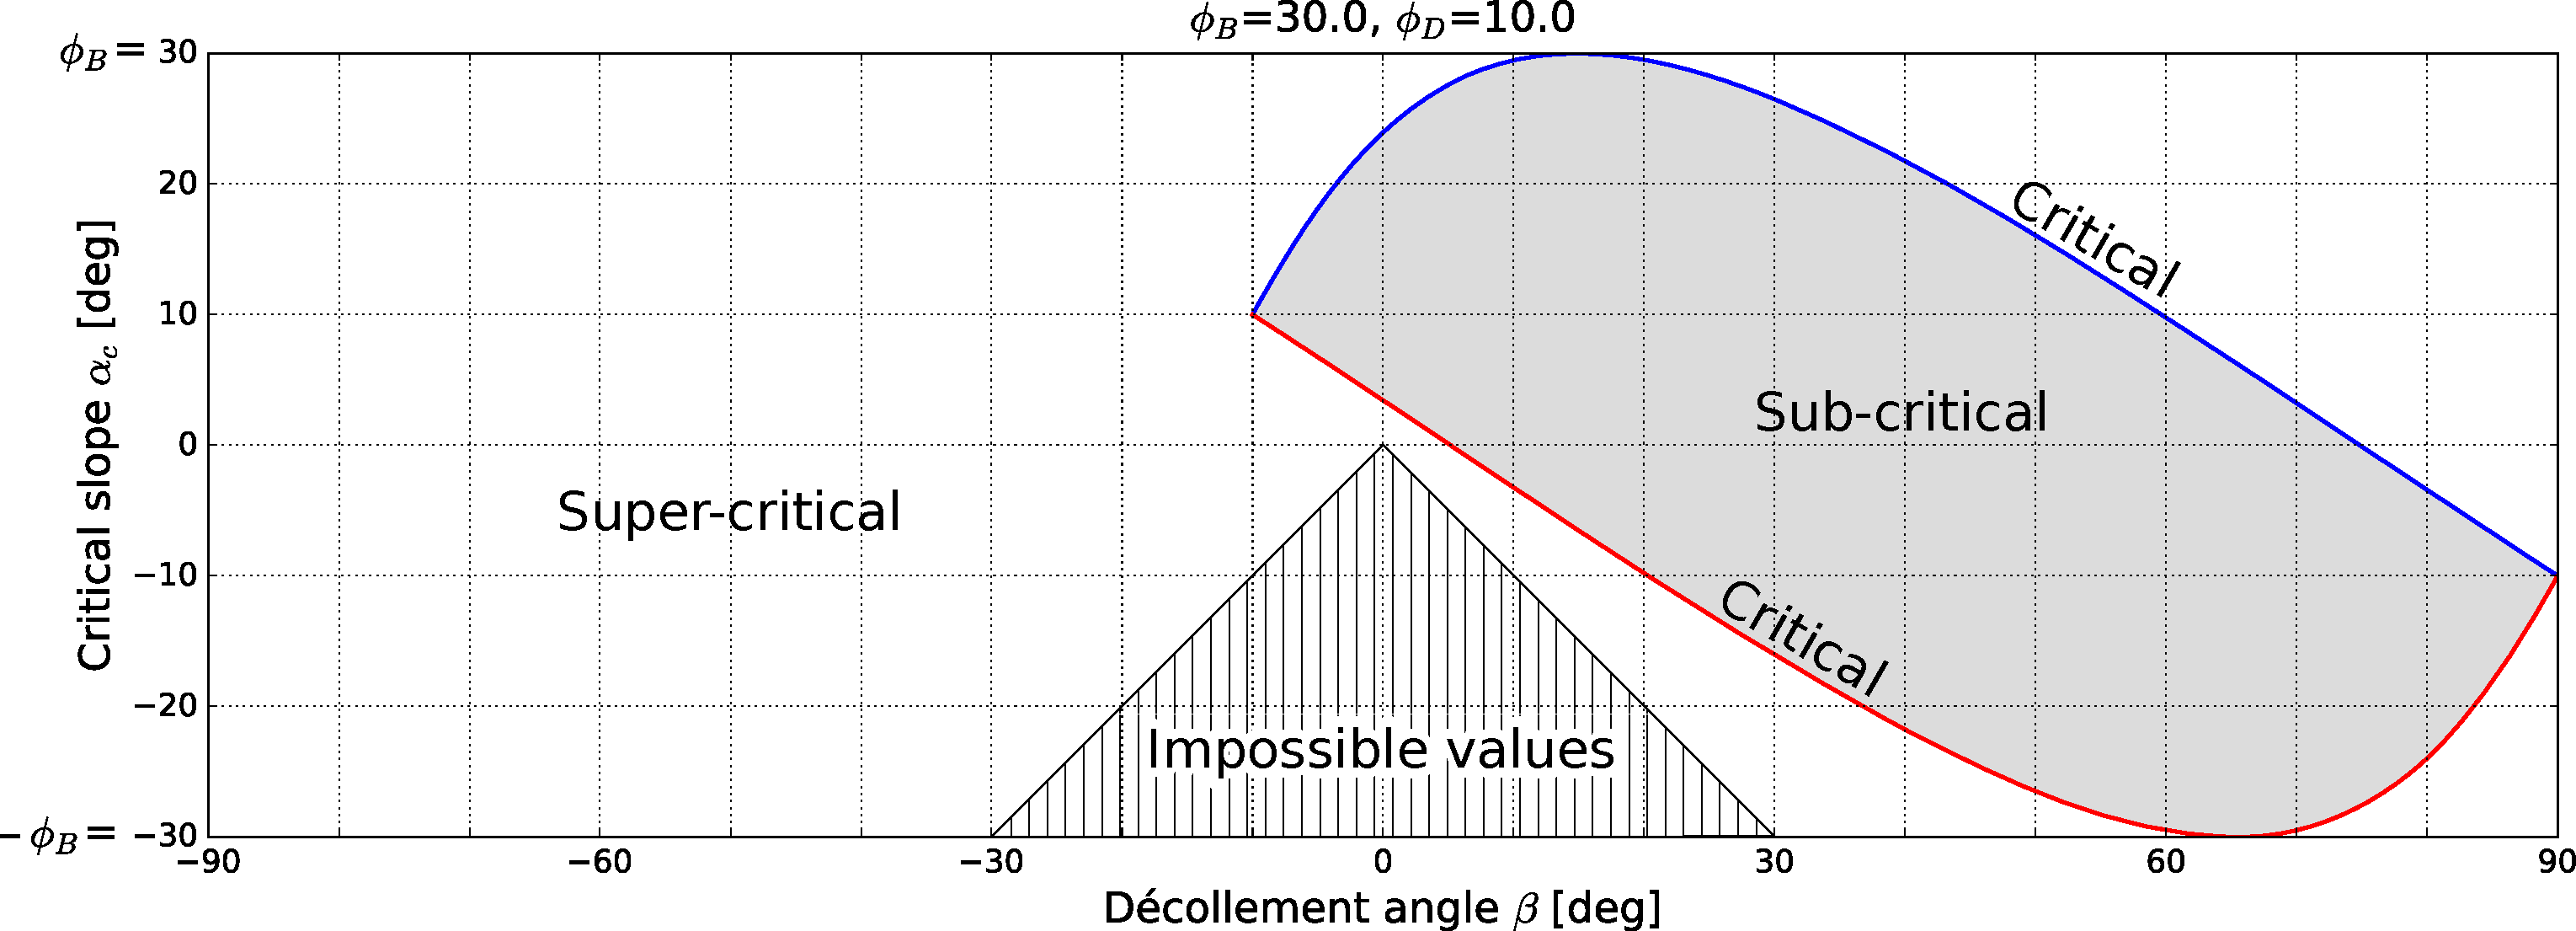
\includegraphics[width=15cm]{ECCW_domains.pdf}
	\caption{The domains of stability defined by the critical enveloppes : deformation occurs in the prism if it lays in the sub-critical domain (gray surface), including the critical enveloppes (red and blue lines). No deformation occurs in the super-critical domain : the tectonic force is accomodated only by sliding on the basal décollement.}
	\label{fig:domains}
\end{figure}





%-----------------------------------------------------------------------------------------------------------
\subsection{Motor of faulting}

Mathematically constituted of four parts due to the two $\arcsin$ included in the impicite solution (see section \ref{sec:compute_ECCW}), the critical enveloppe is meaningfull by group of two.
In all plots of this documentation, the enveloppe is drawed in two parts, highlited by the red and blue lines.
The red line represent configurations where the faults are in reverse mode, while the configurations under the blue line are in normal mode (see Figure \ref{fig:example_section-comp} and \ref{fig:example_section-ext}).

The "motor" of normal or reverse faulting is in all cases tectonic motion or gravitational collapse.
According to the geological context, these "motors" are seted differently.
For compressive context, reverse faulting (bottom red line) is driven by tectonic motion while normal faulting is due to gravitational collapse (Figure \ref{fig:example_section-comp}).
For extensive context this normal faulting (upper blue line) which is driven by tectonic motion and reverse faulting by gravitational collapse (Figure \ref{fig:example_section-ext}).




%-----------------------------------------------------------------------------------------------------------
\newpage
\section{Compute ECCW}
\label{sec:compute_ECCW}
%-----------------------------------------------------------------------------------------------------------

%-----------------------------------------------------------------------------------------------------------
\subsection{Critical prism theory}


From \cite{Dahlen1984} and \cite{Yuan2015} we get a relation between the basal slope $\beta$ and the topographic slope $\alpha$ of a frictional material pushed by an horizontal tectonic force.

%-----------------------------------------------------------------------------------------------------------
\subsection{The exact implicit solution}

From \citep{Yuan2015}, we get :
\begin{equation}
	\alpha_c + \beta = \Psi_D - \Psi_0
	\label{eq:ECCW-implicit} 
\end{equation}
with
\begin{align}
	\Psi_D &= \frac{1}{2} \arcsin \left( \frac{(1 - \lambda_D) \sin(\phi_D)}{(1 - \lambda_B) \sin(\phi_B)} + \frac{\lambda_D - \lambda_B}{1 - \lambda_B} \sin(\phi_D) \cos(2 \Psi_0) \right) - \frac{1}{2} \phi_D
	\label{eq:ECCW-psi_D} \\ 
	\Psi_0 &= \frac{1}{2} \arcsin \left( \frac{\sin(\alpha_c')}{\sin(\phi_B)} \right)  - \frac{1}{2} \alpha_c'
	\label{eq:ECCW-psi_0} \\
	\alpha_c' & = \arctan \left( \frac{1 - \frac{\rho_f}{\rho}}{1 - \lambda_B} \tan(\alpha_c) \right)
	\label{eq:ECCW-alphacp} 
\end{align}


%-----------------------------------------------------------------------------------------------------------
\subsection{Fault slopes at criticality}

\begin{align}
	\theta_{A1} = \gamma_{A2} &= \frac{\pi}{4} + \frac{\phi_B}{2} - \frac{1}{2} \arcsin \left( \frac{\sin(\alpha_c')}{\sin(\phi_B)} \right) - \frac{1}{2} \alpha_c' + \alpha_c
	\label{eq:theta-A} \\
	\gamma_{A1} = \theta_{A2} &= \frac{\pi}{4} + \frac{\phi_B}{2} + \frac{1}{2} \arcsin \left( \frac{\sin(\alpha_c')}{\sin(\phi_B)} \right) + \frac{1}{2} \alpha_c' - \alpha_c
	\label{eq:gamma-A}
\end{align}


\begin{align}
	\theta_{B1} = \gamma_{B2} &= \frac{\pi}{4} - \frac{\phi_B}{2} + \frac{1}{2} \arcsin \left( \frac{\sin(\alpha_c')}{\sin(\phi_B)} \right) - \frac{1}{2} \alpha_c' + \alpha_c
	\label{eq:theta-B} \\
	\gamma_{	B1} = \theta_{B2} &= \frac{\pi}{4} - \frac{\phi_B}{2} - \frac{1}{2} \arcsin \left( \frac{\sin(\alpha_c')}{\sin(\phi_B)} \right) + \frac{1}{2} \alpha_c' - \alpha_c
	\label{eq:gamma-B}
\end{align}

\begin{align}
	\max(\alpha_c) = - \min(\alpha_c) &= \arctan \left( \frac{1 - \lambda_B}{1 - \frac{\rho_w}{\rho}} \tan(\phi_B) \right)
	\label{eq:alphaminmax}\\
\end{align}


\begin{figure}[h]
	\centering
	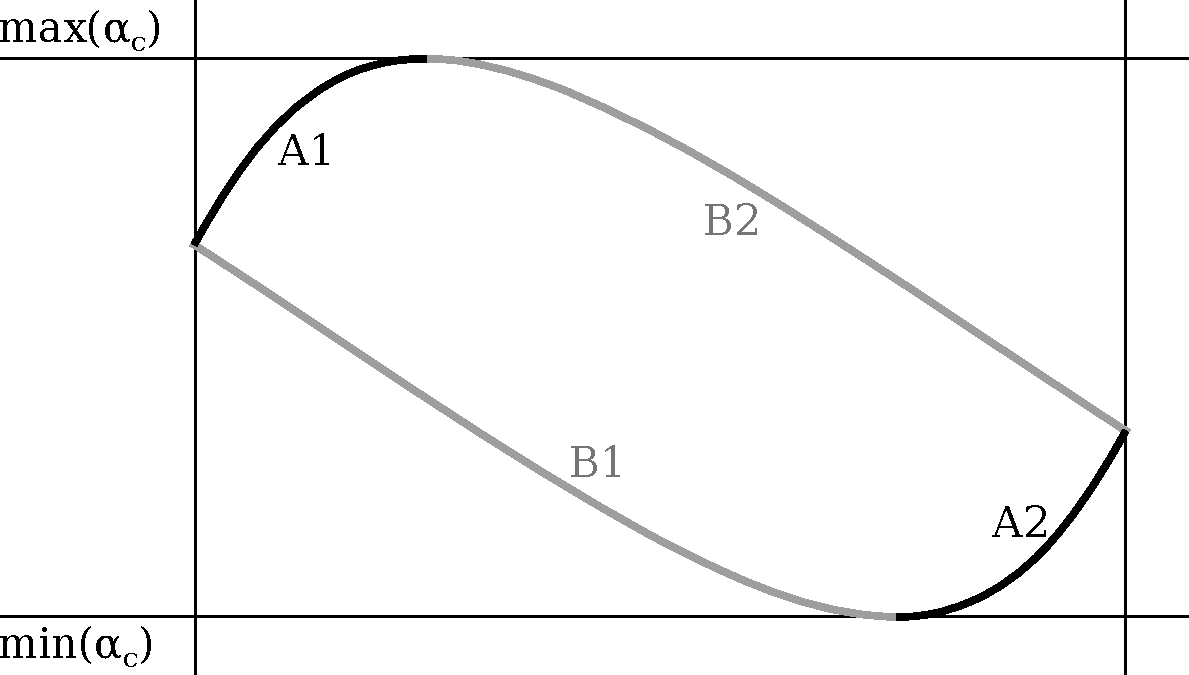
\includegraphics[width=8cm]{ECCW_maths_domains.pdf} 
	\caption{The four mathematic domains of the critical enveloppes.}
	\label{fig:maths-domains}
\end{figure}

%-----------------------------------------------------------------------------------------------------------
\subsection{Solve ECCW}

An iterative method is necessary to solve ECCW. 
Here we had choose Newton's secant method.
But some issues raise when one try to solve (\ref{eq:ECCW-implicit}) directly due to the two $\arcsin$ included in (\ref{eq:ECCW-psi_D}) and (\ref{eq:ECCW-psi_0}).
We choose here to rewrite equations (\ref{eq:ECCW-implicit}), (\ref{eq:ECCW-psi_D}) and (\ref{eq:ECCW-psi_0}) into a set of three functions that should equals zero :
\begin{align}
	f_1 &= \alpha_c + \beta - \Psi_D + \Psi_0
	\label{eq:f1} \\
	f_2 &= \sin(2 \Psi_D + \phi_D) - \frac{(1 - \lambda_D) \sin(\phi_D)}{(1 - \lambda_B) \sin(\phi_B)} - \frac{\lambda_D - \lambda_B}{1 - \lambda_B} \sin(\phi_D) \cos(2 \Psi_0)  
	\label{eq:f2} \\
	f_3 &= \sin(2 \Psi_0 + \alpha_c') \sin(\phi_B) - \sin(\alpha_c')
	\label{eq:f3} 
\end{align}
This set of equation can be used in an adapted form of the Newton's Method.

%-----------------------------------------------------------------------------------------------------------
\subsection{Newton's method}

We use the Newton's secant method to iteratively converge towards the solution.
\\
The iteration :
\begin{equation}
	\Delta x = \frac{f(x_i)}{f'(x_i)}
	\label{eq:newton-iteration}
\end{equation}
with $\Delta_x = x_{i+1} - x_i$ and $f'$ the derivative of $f$.
Iterates until $\Delta x < \epsilon$, an arbitrary small threeshold. 
Initial value $x_0$ is given by user.
\\
The derivative $f'$ can be approximated using finite difference:
\begin{equation}
	f'(x_i) = \frac{f(x_i) - f(x_{i-1})}{x_i - x_{i-1}} 
	\label{eq:fp1}
\end{equation}
or
\begin{equation}
	f'(x_i) = \frac{f(x_i + h) - f(x_i)}{h} 
	\label{eq:fp2}
\end{equation}
with $h$ a an arbitrary small value.

%-----------------------------------------------------------------------------------------------------------
\subsection{Adaptation of Newton's method to a set of functions}

Let's define $\vec{F}$, a set of $n$ functions :
\begin{equation}
	\vec{F} = \left[ \begin{matrix}
		f_1(\vec{X}) \\ 
		\vdots \\ 
		f_n(\vec{X})
	\end{matrix} \right] 
	\label{eq:set_of_functions}
\end{equation}
with $\vec{X} = x_1, \dots, x_n$, $n$ parameters.
The derivative of each subfunction $f_k$ is the sum of the partial derivative on $\vec{X}$. 
It is convenient for what follows to define $\mat{M}$, a $n \times n$ matrix, constituted of partial derivative on $\vec{X}$ for columns, with lines dedicated to subfunctions :
\begin{equation}
	\mat{M} = \left[ \begin{matrix}
	\frac{\partial f_1}{\partial x_1} & \hdots & \frac{\partial f_1}{\partial x_n} \\ 
	\vdots & \ddots  & \vdots \\ 
	\frac{\partial f_n}{\partial x_1} & \hdots & \frac{\partial f_n}{\partial x_n}
	\end{matrix}  \right] 
	\label{eq:matrix_of_derivatives}
\end{equation}
Each elements of $\mat{M}$ can be approximated using (\ref{eq:fp1}) or (\ref{eq:fp2}). 
For example, using  (\ref{eq:fp2}) on a set of 3 equations function of $\vec{X} = (x, y, z)$, $\mat{M}(\vec{X_i})$  is given by
\begin{equation}
	\left[ \begin{matrix}
	\frac{f_1(x_i + h, y_i, z_i) - f_1(\vec{X_i})}{h} & \frac{ f_1(x_i, y_i + h, z_i) - f_1(\vec{X_i})}{h} & \frac{ f_1(x_i, y_i, z_i + h) - f_1(\vec{X_i})}{h} \\ 
	\frac{ f_2(x_i + h, y_i, z_i) - f_2(\vec{X_i})}{h} & \frac{ f_2(x_i, y_i + h, z_i) - f_2(\vec{X_i})}{h} & \frac{ f_2(x_i, y_i, z_i + h) - f_2(\vec{X_i})}{h} \\ 
	\frac{ f_3(x_i + h, y_i, z_i) - f_3(\vec{X_i})}{h} & \frac{ f_3(x_i, y_i + h, z_i) - f_3(\vec{X_i})}{h} & \frac{ f_3(x_i, y_i, z_i + h) - f_3(\vec{X_i})}{h}
	\end{matrix}    \right]
	\label{eq:matrix_of_derivatives-example} 
\end{equation}
Using (\ref{eq:set_of_functions}) and (\ref{eq:matrix_of_derivatives}), we can now rewrite (\ref{eq:newton-iteration}) :
\begin{gather}
	\mat{M} \cdot \Delta \vec{X} = - \vec{F}
	\label{eq:newton-iteration-matrix1} \\
	\Delta \vec{X} = \mat{M}^{-1} \cdot - \vec{F}
	\label{eq:newton-iteration-matrix2}	
\end{gather}
This last rewriting allows to solve \ref{eq:f1}, \ref{eq:f2} and \ref{eq:f3} by iteration, using $\vec{X} = (\beta, \Psi_0, \Psi_D)$.


%----------------------------------------------------- Appendix C 

\clearpage
%\end{appendix}

%----------------------------------------------------- References --------------------------------------------------------------------------
%-------------------------------------------------------------------------------------------------------------------------------------------------
%------------------------------------------------------------------------------------------------------------------------------------------------
%--------------- BIBLIOGRAPHY----------------------------------------------------------------------------------------------------------
\bibliographystyle{apalike}
\bibliography{BIBLIO}

%----------------That's all Folks !  ---------------------------------------------------------------------------------
\end{document}

